\chapter{Validierung}
\label{cha:Validierung}

In diesem Kapitel testen wir die Lernfähigkeit und die Lerndauer des TD-Q Agenten, in der Strategiespielumgebung 9 und 16 Spielfelder Tic Tac Toe. Wir testen ebenso die Spielstärke des vorausschauenden Tic Tac Toe Heuristik Agenten. Der TD-Q-Agent und der Heuristik Agent spielen genau 100 Testspiele gegeneinander und 100 Testspiele gegen einen Zufallsagenten. \\

Der TD-Q Agent wird 3 verschiedene Lernphasen ausführen. Die Lernphasen unterscheiden sich in der Anzahl der Trainingsspiele. Untersucht werden vom TD-Q Agenten gelernte Strategien, die in 100 Trainingsspielen (Lernphase 1), in 1.000 Trainingsspielen (Lernphase 2) und in 10.000 Trainingsspielen (Lernphase 3), gegen sich selbst trainiert werden. Jede dieser Lernphasen wird für das 9 Spielfelder Tic Tac Toe und das 16 Spielfelder Tic Tac Toe ausgeführt. \\

Im nächsten Kapitel \ref{cha:Auswertung} werden wir erklären warum wir den TD-Q-Agenten keine Strategie für Reversi lernen lassen. Die Ergebnisse der Tests für das 9 Spielfelder Tic Tac Toe und das 16 Spielfelder Tic Tac Toe werden diese Erklärung belegen. \\

Die für das Testen der Agenten implementierten Strategiespielumgebungen wurden mit dem Python Paket ''unittest'' getestet. Die Tests der Tic Tac Toe Strategiespielumgebung befinden sich in der Datei ''TestTicTacToe.py'' und die Tests der Reversi Strategiespielumgebung befinden sich in der Datei ''TestReversi.py''. In diesen Dateien sind die wichtigsten Funktionalitäten der Strategiespielumgebungen ausgeführt und mit ''asserts'' getestet. Alle Tests der Strategiespielumgebungen waren positiv und könnten bei Bedarf wiederholt werden. \\

\begin{figure}[!htbp]
  \centering
  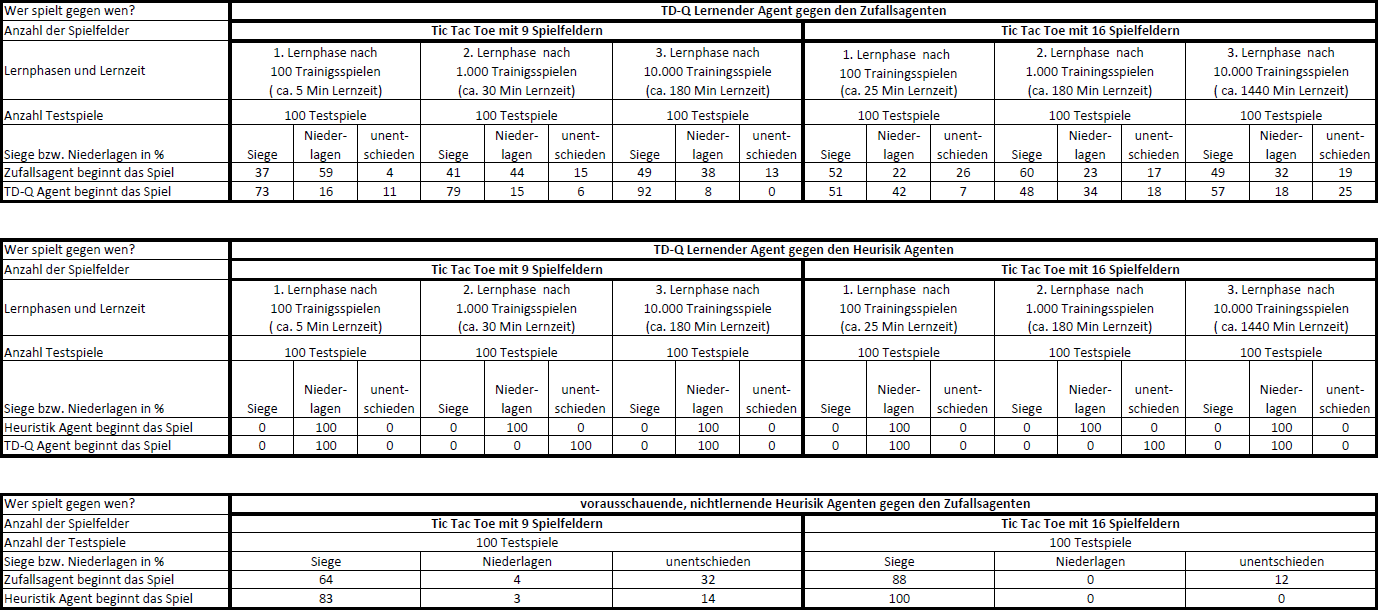
\includegraphics[angle = 90, scale = 0.8]{inhalt/abbildungen/testergebnisse.png}
  \caption{Die Ergebnisse der Agententests.}
  \label{fig:Ergebnisse der Agententests}
\end{figure} 